\begin{frame}{RISULTATI SPERIMENTALI - PRUNING}
    \begin{minipage}{\linewidth}
        \vspace{-.14cm}
        \centering
        \begin{minipage}{0.45\linewidth}
            \begin{figure}
                \centering
                \hspace*{-2.5cm}
                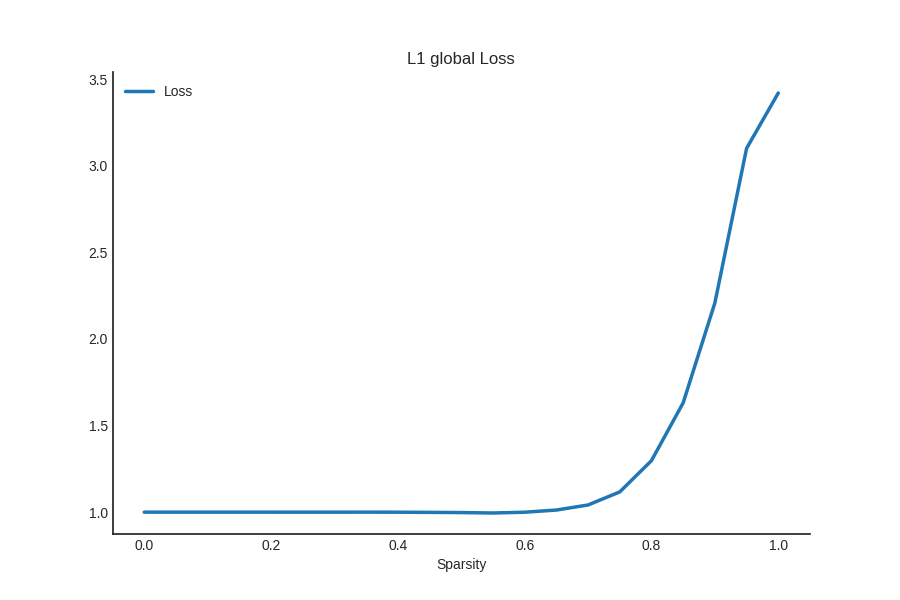
\includegraphics[width = 1.35\linewidth]{global_Loss.png}
                \centering
                %\caption{Perdita classificazione Global Unstructured Pruning.}
            \end{figure}
        \end{minipage}
        \hspace*{-1cm}
        \begin{minipage}{0.50\linewidth}
            \begin{center}
                \resizebox{1.25\textwidth}{!}{%
                  \begin{tabular}{|M{1.5cm}||M{1.3cm}|M{1.3cm}||M{1.3cm}|M{1.3cm}||M{1.3cm}|M{1.3cm}|} 
                    \multicolumn{7}{l}{\hspace{0.6cm} \textbf{Tabella: } Differenza (D) percentuale della perdita (L) a sparsità variabile.} \\ 
                    \hline
                    \multirow{2}{*}{\bfseries{\small SPARSITY}} & \multicolumn{2}{c||}{\bfseries{G-LOSS}} & \multicolumn{2}{c||}{\bfseries{R-LOSS}} & \multicolumn{2}{c|}{\bfseries{C-LOSS}}\\  & {\bfseries{L}} & \bfseries{D}  & \bfseries{L} & \bfseries{D} & \bfseries{L} & \bfseries{D} \\                     
                    \hline
                    \hline
                    {\bfseries{0\%}} & 3.20 & / & 1.03 & / & 2.17 & / \\
                    \hline
                    {\bfseries{20\%}} & 3.20 & \color{Green}{{\bfseries{0\%}}} & 1.03 & \color{Green}{{\bfseries{0\%}}} & 2.17 & \color{Green}{{\bfseries{0\%}}}\\
                    \hline 
                    {\bfseries{40\%}} & 3.20 & \color{Green}{{\bfseries{0\%}}} & 1.03 & \color{Green}{{\bfseries{0\%}}} & 2.17 & \color{Green}{{\bfseries{0\%}}}\\
                    \hline
                    {\bfseries{60\%}} & 3.22 & \color{Green}{{\bfseries{0.62\%}}} & 1.06 & \color{Green}{{\bfseries{2.91\%}}} & 2.16 & \color{Green}{{\bfseries{-0.46\%}}}\\
                    \hline
                    \hline
                    {\bfseries{80\%}} & 4.15 & \color{red}{{\bfseries{29.69\%}}} & 1.27 & \color{red}{{\bfseries{23.3\%}}} & 2.88 & \color{red}{{\bfseries{32.72\%}}}\\
                    \hline
                    {\bfseries{90\%}} & 7.06 & \color{red}{{\bfseries{120.6\%}}} & 2.17 & \color{red}{{\bfseries{110.7\%}}} & 4.89 & \color{red}{{\bfseries{125.3\%}}}\\
                    \hline
                    {\bfseries{100\%}} & 10.95 & \color{red}{{\bfseries{242.2\%}}} & 2.72 & \color{red}{{\bfseries{164.1\%}}} & 8.23 & \color{red}{{\bfseries{279.3\%}}}\\
                    \hline
                 \end{tabular}}
            \end{center} 
        \end{minipage}
    \end{minipage}
    \begin{minipage}{\linewidth}
        \centering
        \begin{minipage}{0.45\linewidth}
            %\vspace{-.4cm}
            \begin{figure}
                \centering
                \hspace*{-1.3cm}
                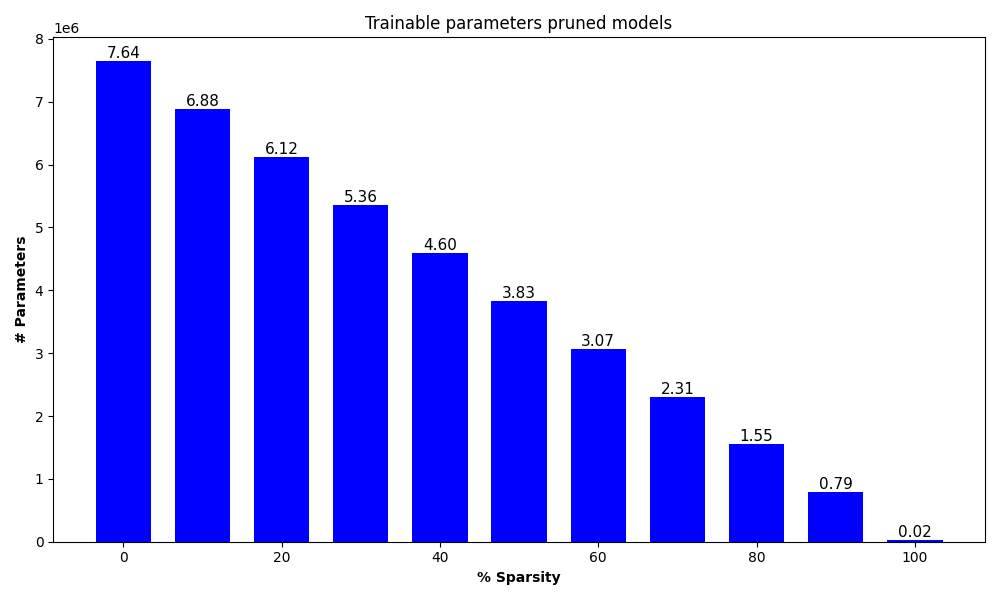
\includegraphics[width = 1.2\linewidth]{Pruning_Unstructured_parameters.png}
                \centering
                %\caption{Riduzione del numero di parametri via pruning a sparsità variabile.}
                \label{par_pruning}
            \end{figure}
        \end{minipage}
        $\Rightarrow$
        \begin{minipage}{0.45\linewidth}
            \begin{figure}
                \centering
                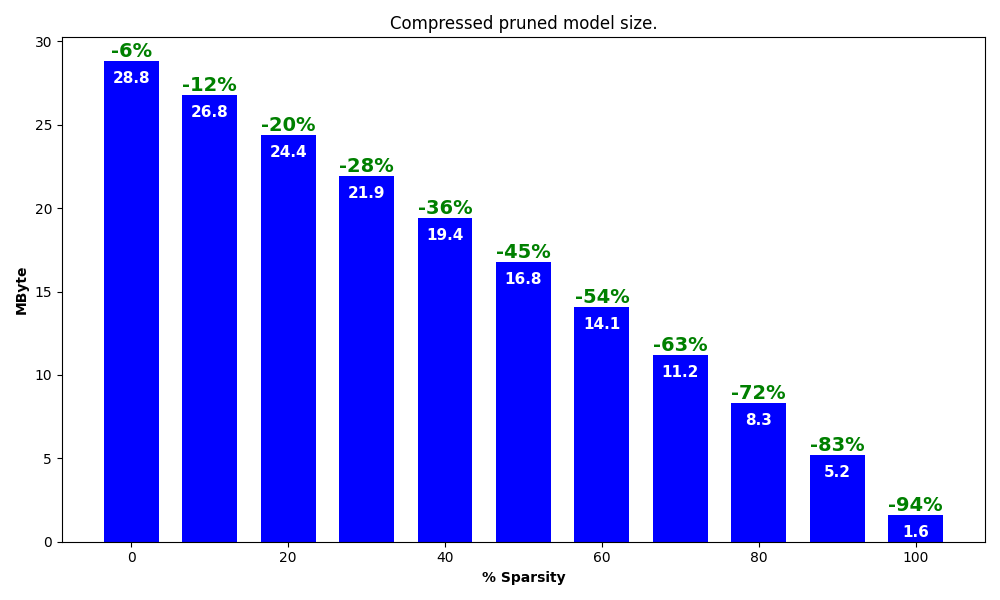
\includegraphics[width = 1.2\linewidth]{Unstructured_size_reduction.png}
                \centering
                %\caption{Riduzione della dimensione del modello SSD via pruning tramite l'utility \emph{gzip}.}
                %\label{SSD_dim}
            \end{figure}
        \end{minipage}
    \end{minipage}

\end{frame}